\bta{研究电磁感应现象}




\begin{enumerate}
%\renewcommand{\labelenumi}{\arabic{enumi}.}
% A(\Alph) a(\alph) I(\Roman) i(\roman) 1(\arabic)
%设定全局标号series=example	%引用全局变量resume=example
%[topsep=-0.3em,parsep=-0.3em,itemsep=-0.3em,partopsep=-0.3em]
%可使用leftmargin调整列表环境左边的空白长度 [leftmargin=0em]
\item	
\exwhere{$ 2019 $ 年 $ 4 $ 月浙江物理选考}
在“探究电磁感应的产生条件”实验中,实验连线后如图 $ 1 $ 所示,感应
线圈组的内外线圈的绕线方向如图 $ 2 $ 粗线所示。
% TODO: \usepackage{graphicx} required
\begin{figure}[h!]
\centering
\begin{subfigure}{0.4\linewidth}
\centering
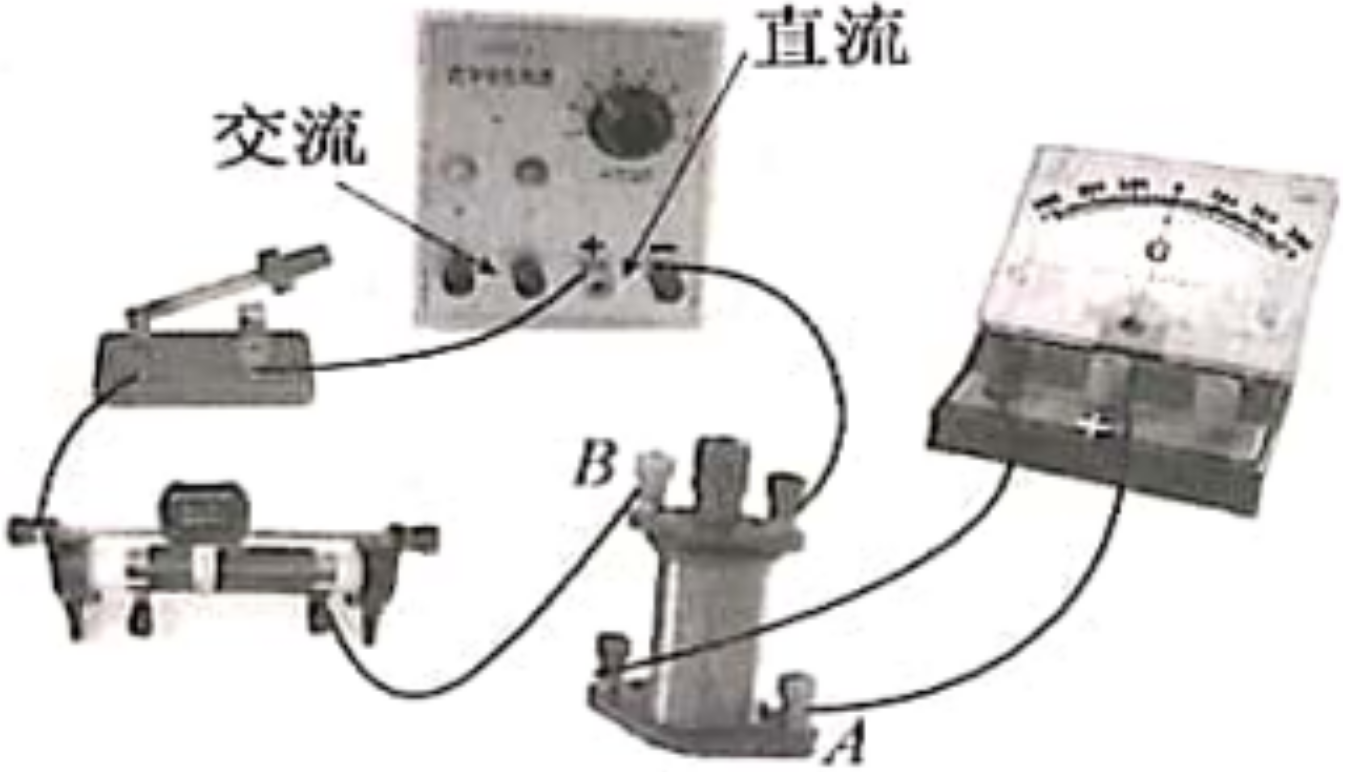
\includegraphics[width=0.87\linewidth]{picture/screenshot062}
\caption{}\label{}
\end{subfigure}
\begin{subfigure}{0.4\linewidth}
\centering
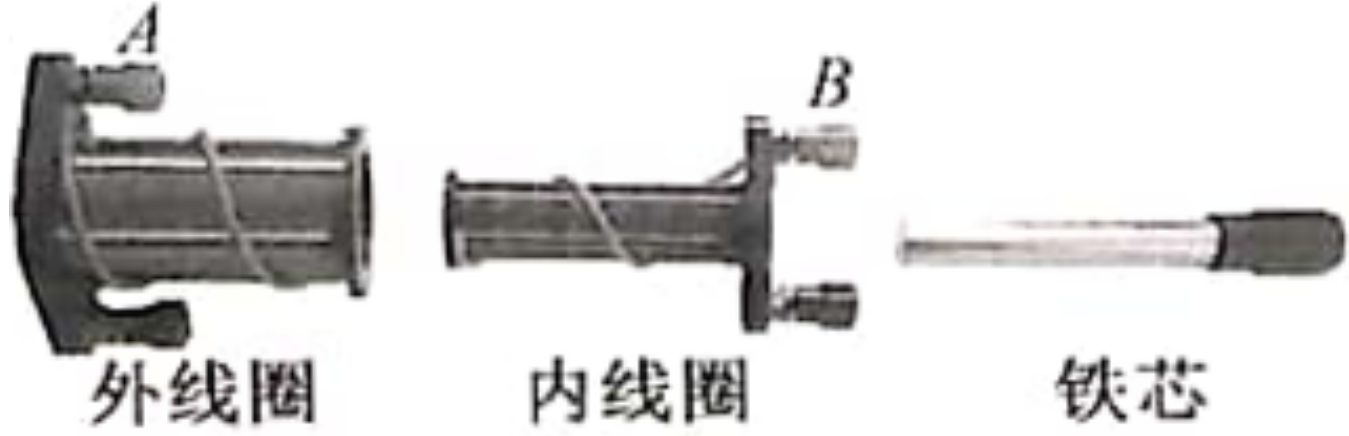
\includegraphics[width=0.8\linewidth]{picture/screenshot063}
\caption{}\label{}
\end{subfigure}
\end{figure}



\begin{enumerate}
%\renewcommand{\labelenumi}{\arabic{enumi}.}
% A(\Alph) a(\alph) I(\Roman) i(\roman) 1(\arabic)
%设定全局标号series=example	%引用全局变量resume=example
%[topsep=-0.3em,parsep=-0.3em,itemsep=-0.3em,partopsep=-0.3em]
%可使用leftmargin调整列表环境左边的空白长度 [leftmargin=0em]
\item
接通电源,闭合开关,$ G $ 表指针会有大的偏转,几秒后 $ G $ 表指针停在中间不动。将滑动变阻
器的触头迅速向右滑动时,$ G $ 表指针 \underlinegap (“不动”、“右偏”、“左偏”、“不停振动”);迅速抽出铁芯
时,$ G $ 表指针 \underlinegap (“不动”、“右偏”、“左偏”、“不停振动”)。

\item 
断开开关和电源,将铁芯重新插入内线圈中,把直流输出改为交流输出,其他均不变。接通
电源,闭合开关,$ G $ 表指针 \underlinegap (“不动”、“右偏”、“左偏”、“不停振动”)。

\item 
仅用一根导线,如何判断 $ G $ 表内部线圈是否断了?

\hfullline 

\end{enumerate}

\tk{
\begin{enumerate}
%\renewcommand{\labelenumi}{\arabic{enumi}.}
% A(\Alph) a(\alph) I(\Roman) i(\roman) 1(\arabic)
%设定全局标号series=example	%引用全局变量resume=example
%[topsep=-0.3em,parsep=-0.3em,itemsep=-0.3em,partopsep=-0.3em]
%可使用leftmargin调整列表环境左边的空白长度 [leftmargin=0em]
\item
左偏 \quad 右偏
\item 
不停振动
\item 
短接 $ G $ 表前后各摇动 $ G $ 表一次,比较指针偏转,有明显变化,则线圈断了;没有明显偏转则未断。
\end{enumerate}
} 






\item
\exwhere{$ 2013 $ 年上海卷}
演示地磁场存在的实验装置(由环形线圈,微电流传感器,$ DIS $ 等组成)如图所示。首
先将线圈竖直放置,以竖直方向为轴转动,屏幕上的电流指针 \underlinegap 
(填:“有”或“无”)偏转;然后仍将线圈竖直放置,使其平面与东西向
平行,并从东向西移动,电流指针
\underlinegap 
(填:“有”或“无”)偏转;最
后将线圈水平放置,使其从东向西移动,电流指针
\underlinegap 
(填:“有”或“无”)偏转。
% TODO: \usepackage{graphicx} required
\begin{figure}[h!]
\centering
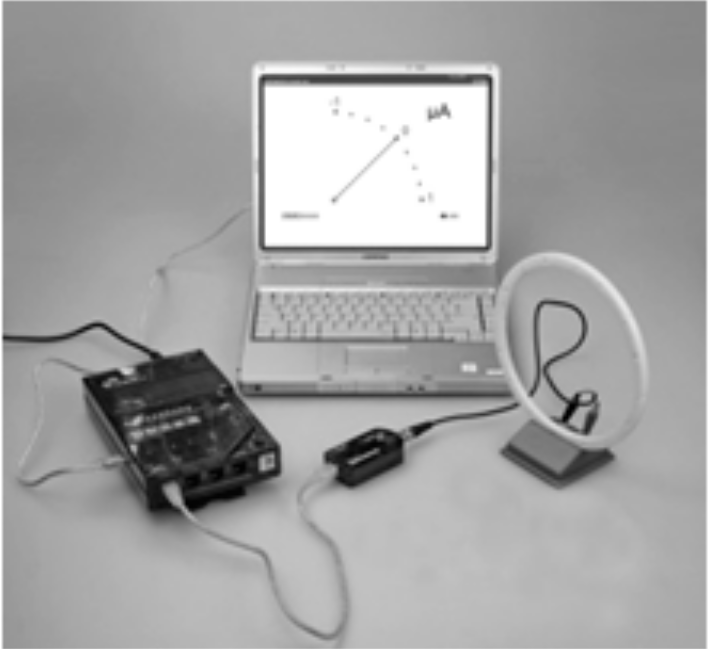
\includegraphics[width=0.23\linewidth]{picture/screenshot064}
\end{figure}

\tk{有 \quad 无 \quad 无} 



\item 
\exwhere{$ 2012 $ 年物理上海卷}
为判断线圈绕向,可将灵敏电流计 $ G $ 与线圈 $ L $ 连接,如
图所示。己知线圈由 $ a $ 端开始绕至 $ b $ 端:当电流从电流计 $ G $ 左端流入
时,指针向左偏转。
\begin{enumerate}
%\renewcommand{\labelenumi}{\arabic{enumi}.}
% A(\Alph) a(\alph) I(\Roman) i(\roman) 1(\arabic)
%设定全局标号series=example	%引用全局变量resume=example
%[topsep=-0.3em,parsep=-0.3em,itemsep=-0.3em,partopsep=-0.3em]
%可使用leftmargin调整列表环境左边的空白长度 [leftmargin=0em]
\item
将磁铁 $ N $ 极向下从线圈上方竖直插入 $ L $ 时,发现指针向左偏转。
俯视线圈,其绕向为 \underlinegap (填:“顺时针”或“逆时针”)
。

\item 
当条形磁铁从图中的虚线位置向右远离 $ L $ 时,指针向右偏转。
俯视线圈,其绕向为 \underlinegap (填:“顺时针”或“逆时针”)
。

\end{enumerate}
\begin{figure}[h!]
\centering
\includesvg[width=0.23\linewidth]{picture/svg/GZ-3-tiyou-1036}
\end{figure}

\tk{
\begin{enumerate}
%\renewcommand{\labelenumi}{\arabic{enumi}.}
% A(\Alph) a(\alph) I(\Roman) i(\roman) 1(\arabic)
%设定全局标号series=example	%引用全局变量resume=example
%[topsep=-0.3em,parsep=-0.3em,itemsep=-0.3em,partopsep=-0.3em]
%可使用leftmargin调整列表环境左边的空白长度 [leftmargin=0em]
\item
顺时针
\item 
逆时针
\end{enumerate}
} 



\item 
\exwhere{$ 2011 $年上海卷}
在“研究回路中感应电动势大
小与磁通量变化快慢的关系”实验(见图
$ (a) $)中,得到$ E-1/ \Delta t $ 图线如图$ (b) $所示。
\begin{figure}[h!]
\centering
\begin{subfigure}{0.4\linewidth}
\centering
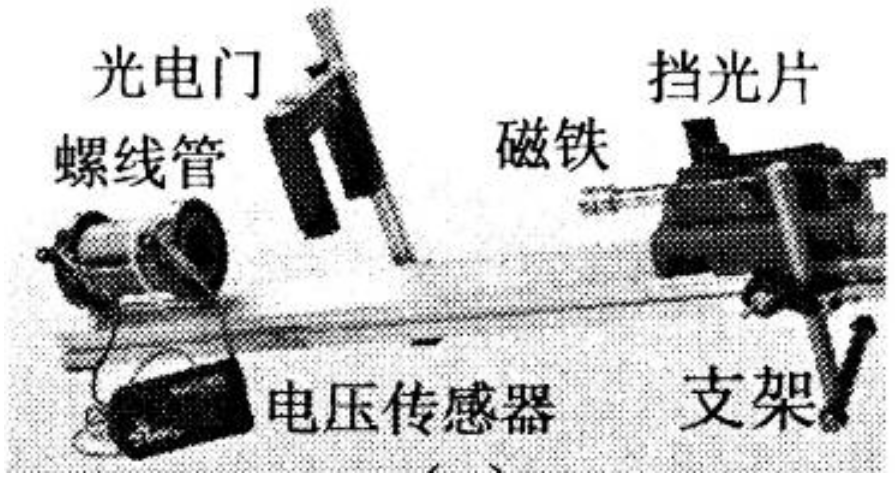
\includegraphics[width=0.7\linewidth]{picture/screenshot065}
\caption{}\label{}
\end{subfigure}
\begin{subfigure}{0.4\linewidth}
\centering
\includesvg[width=0.7\linewidth]{picture/svg/GZ-3-tiyou-1037} 
\caption{}\label{}
\end{subfigure}

\end{figure}


\begin{enumerate}
%\renewcommand{\labelenumi}{\arabic{enumi}.}
% A(\Alph) a(\alph) I(\Roman) i(\roman) 1(\arabic)
%设定全局标号series=example	%引用全局变量resume=example
%[topsep=-0.3em,parsep=-0.3em,itemsep=-0.3em,partopsep=-0.3em]
%可使用leftmargin调整列表环境左边的空白长度 [leftmargin=0em]
\item
(多选题)在实验中需保持不变的是 \underlinegap 。
\fourchoices
{挡光片的宽度}
{小车的释放位置}
{导轨倾斜的角度}
{光电门的位置}


\item 
线圈匝数增加一倍后重做该实验,在图$ (b) $中画出实验图线。



\end{enumerate}

\tk{
\begin{enumerate}
%\renewcommand{\labelenumi}{\arabic{enumi}.}
% A(\Alph) a(\alph) I(\Roman) i(\roman) 1(\arabic)
%设定全局标号series=example	%引用全局变量resume=example
%[topsep=-0.3em,parsep=-0.3em,itemsep=-0.3em,partopsep=-0.3em]
%可使用leftmargin调整列表环境左边的空白长度 [leftmargin=0em]
\item
AD
\item 
如图
\begin{center}
 \includesvg[width=0.23\linewidth]{picture/svg/GZ-3-tiyou-1038} 
\end{center}
\end{enumerate}
} 







\end{enumerate}

